\documentclass[smaller]{beamer}
\usepackage{colortbl}

\usepackage{amsmath}
\usepackage{amssymb}
\usepackage{color}

\renewcommand{\familydefault}{\sfdefault}

% syntactic coloring
% by default, beamer-colors are
%    normal text is black on white.
%    alerted text is red.
%    example text is a dark green (green with 50% black).
%    structure is set to a light version of MidnightBlue (more precisely, 20% red, 20% green, and 70% blue).

\setbeamercolor{key point}{parent=alerted text}

\def\struct{\usebeamercolor[fg]{structure}}
\def\key{\em \usebeamercolor[fg]{key point}}
\def\aside{\scriptsize \usebeamercolor[fg]{example text}}
\def\newthing{\usebeamercolor[fg]{key point}}
\def\oldthing{\usebeamercolor[fg]{structure}}
\def\defthing{\usebeamercolor[fg]{structure}}

% \definecolor{blue}{rgb}{0.05,0.6,1}
% \definecolor{orange}{rgb}{1,0.549,0}
% \definecolor{dark-red}{rgb}{.4,.1,.1}
% \definecolor{pink}{rgb}{1,.8,.8}
% \definecolor{dark-green}{rgb}{.1,.6,.1}
% \definecolor{light-green}{rgb}{.8,1,.8}
% \definecolor{blue-white}{rgb}{.95,.95,1}
% \definecolor{purple}{rgb}{1, 0.0, 0.6}

\newcommand{\R}{\mathbb{R}}
\newcommand{\Q}{\mathbb{Q}}
\newcommand{\Z}{\mathbb{Z}}
\newcommand{\N}{\mathbb{N}}
\newcommand{\C}{\mathbb{C}}

\renewcommand{\P}{\mathbb{P}}
\newcommand{\E}{\mathbb{E}}

\newcommand{\var}{\mathop{\mbox{Var}}}
\newcommand{\cov}{\mathop{\mbox{cov}}}
\newcommand{\median}{\mathop{\mbox{median}}}
%\newcommand{\det}{\mathop{\mbox{det}}}
\newcommand{\supp}{\mathop{\mbox{supp}}}
\newcommand{\sgn}{\mathop{\mbox{sgn}}}

\newcommand{\conv}{\mathop{\mbox{conv}}}
\newcommand{\deq}{\stackrel{\scriptscriptstyle{d}}{=}}
\newcommand{\dcv}{\stackrel{\scriptscriptstyle{d}}{\longrightarrow}}


\newcommand{\figcredit}[1]{{\begin{flushright}\usebeamercolor[fg]{structure} \it \tiny #1 \end{flushright}}}



% plr macros: these are for boxes in tables
\newcommand\tLL[1]{\multicolumn{1}{|c}{#1}}
\newcommand\tRR[1]{\multicolumn{1}{c|}{#1}}
\newcommand\tLR[1]{\multicolumn{1}{|c|}{#1}}

% This file is a solution template for:

% - Giving a talk on some subject.
% - The talk is between 15min and 45min long.
% - Style is ornate.



% Copyright 2004 by Till Tantau <tantau@users.sourceforge.net>.
%
% In principle, this file can be redistributed and/or modified under
% the terms of the GNU Public License, version 2.
%
% However, this file is supposed to be a template to be modified
% for your own needs. For this reason, if you use this file as a
% template and not specifically distribute it as part of a another
% package/program, I grant the extra permission to freely copy and
% modify this file as you see fit and even to delete this copyright
% notice. 

\def\typezero{\circ}
\def\typeone{\bullet}

\setbeamertemplate{blocks}[default]
\usecolortheme{rose}

\mode<presentation>
{
  % \usetheme{default}
  \usetheme{boxes}
  % or ...
  \usefonttheme[options]{structuresmallcapsserif}

  \setbeamercovered{transparent}
  % or whatever (possibly just delete it)
}


\usepackage[english]{babel}
% or whatever

\usepackage[latin1]{inputenc}
% or whatever

\usepackage{times}
\usepackage[T1]{fontenc}
% Or whatever. Note that the encoding and the font should match. If T1
% does not look nice, try deleting the line with the fontenc.


\title[Context-dependent models] % (optional, use only with long paper titles)
{Context-dependent models of nucleotide substitution}

\author % (optional, use only with lots of authors)
{Peter Ralph}
% - Use the \inst{?} command only if the authors have different
%   affiliation.

\institute[USC]
{
  USC -- Computational Biology and Bioinformatics
  }
% - Use the \inst command only if there are several affiliations.
% - Keep it simple, no one is interested in your street address.

\date % (optional)
{October 14, 2013\\Bartolom\'e Day}


\begin{document}


% Abstract: 
% It is well-known that the nucleotide mutation process is context-dependent:
% the probability of change at a particular base depends not only on the
% nucleotide at that position, but also at its neighbors; CpG hypermutability
% is the most well-known such effect.  Selection for or against particular
% motifs adds more layers of context dependencies to the nucleotide
% substitution process.  Incorporating context dependence is difficult, because
% this in principle requires summing over all possible substitutions at all
% sites.  I will present a computaionally feasible method to do these
% calculations correctly, which enables Bayesian inference of phylogenetic
% branch lengths, mutation rates, and selection coefficients of short motifs.
% I will also illustrate with examples to some models of statistical physics,
% such as estimation of the magnetization and temperature in the Ising model.

\begin{frame}
  \titlepage
\end{frame}


%%%%
% OUTLINE
%
% Intro to the problem
%   statement of the problem
%      mutation + selection
%   artificial example: TASEP
%   propagation of dependency
%   e^{tG}
%   previous work
%
% Method
%   restrict to pattern frequencies: partial likelihood
%   still missing edge effects: marginalize over window
%     node average boundary
%   asymptotically correct: propagation of dependency
%   likelihood function
%   computation: sparse matrices
%   phylogenetic peeling (?)
%
% Applications
%   TASEP
%   CpG
%   Ising
%   real data?
%   ancestral state reconstruction


%%%%%%%%% INTRO
\section{Introduction \& Background}

\begin{frame}{The problem: context dependence}

  \begin{columns}[c]
    \begin{column}{.4\textwidth}

      {\struct Data:} Long (nucleotide) sequences separated by (evolutionary) time \\
        with known (phylogenetic) relationship.

        \vspace{2em}

      {\struct Goal:} Infer properties of the model:\\
        substitution rates; relative amounts of time.

        \vspace{2em}

      {\struct Example:} Each site evolves independently \ldots

    \end{column}
    \begin{column}{.6\textwidth}

      schematic of sequences evolving on the tree

    \end{column}
  \end{columns}

\end{frame}


\begin{frame}{Substitution: mutation $+$ selection}

  {\struct Formal-ish description:}

  \begin{itemize}

    \item {\newthing Mutation} rules $(a_i,b_i,r_i)$: \\
      locations matching $a_i$ mutate to $b_i$ at rate $r_i$

    \item {\newthing Fixation} function: \\
      mutations take effect with probability $f(s(\text{new}) - s(\text{old}))$, \\
      e.g.\ $f(x) = N_e (1-e^{-2 ds})/(1-\exp{-2 N_e ds})$

    \item {\newthing Selection} rules $(u_i,s_i)$: for sequence $x$,\\
      $s(x) = \sum_i s_i n_i(x)$, with $n_i(x)$ number of times $u_i$ matches in $x$
      

  \end{itemize}

\end{frame}

\begin{frame}{Example}

  \begin{columns}[c]
    \begin{column}{.5\textwidth}
  Rules:
  \begin{itemize}
    \item $\text{X} \to \text{O}$ at rate 1
    \item $\text{O} \to \text{X}$ at rate 1
    \item $\text{OX} \to \text{XO}$ at rate $\gamma$
    \item $s(\text{O}) = 1$ and $s(\text{X}) = 0$
  \end{itemize}

    \end{column}
    \begin{column}{.5\textwidth}

      Rate at which OXO $\to$ OXX is
      \begin{align*}
      \gamma \, f( s(\text{OOX}) - s(\text{OXX}) ) &= \gamma \, f( -1 ) 
      \end{align*}
      and OXO $\to$ OOX is
      \begin{align*}
      \gamma \, f( s(\text{OOX}) - s(\text{OXO}) ) &= \gamma \, f( 0 ) .
      \end{align*}

    \end{column}
  \end{columns}

  { \scriptsize
\begin{center} \setlength{\tabcolsep}{0pt} \begin{tabular}{cccccccccccccccccccccccccccccccccccccccccccccccccccccccccccccccccccccccccccccccccccccccccccccccccccccc}
O&O&O&O&X&O&O&X&X&X&O&O&O&O&X&O&O&O&X&O&X&O&O&O&O&O&X&O&O&O&O&O&O&O&O&X&X&O&X&O&O&O&O&X&O&O&O&X&O&O\\
$\centerdot$&$\centerdot$&$\centerdot$&$\centerdot$&$\centerdot$&$\centerdot$&$\centerdot$&$\centerdot$&$\centerdot$&$\centerdot$&$\centerdot$&$\centerdot$&$\centerdot$&$\centerdot$&$\centerdot$&$\centerdot$&$\centerdot$&$\centerdot$&$\centerdot$&$\centerdot$&$\centerdot$&$\centerdot$&$\centerdot$&$\centerdot$&$\centerdot$&$\centerdot$&$\centerdot$&$\centerdot$&$\centerdot$&$\centerdot$&$\centerdot$&$\centerdot$&$\centerdot$&$\centerdot$&$\centerdot$&$\centerdot$&$\centerdot$&$\centerdot$&$\centerdot$&$\centerdot$&$\centerdot$&$\centerdot$&$\centerdot$&$\centerdot$&$\centerdot$&$\centerdot$&$\centerdot$&$\centerdot$&$\centerdot$&$\centerdot$\\
$\centerdot$&$\centerdot$&$\centerdot$&$\centerdot$&$\centerdot$&$\centerdot$&$\centerdot$&$\centerdot$&$\centerdot$&$\centerdot$&$\centerdot$&$\centerdot$&$\centerdot$&$\centerdot$&$\centerdot$&$\centerdot$&$\centerdot$&$\centerdot$&$\centerdot$&$\centerdot$&$\centerdot$&$\centerdot$&$\centerdot$&$\centerdot$&$\centerdot$&$\centerdot$&$\centerdot$&$\centerdot$&$\centerdot$&$\centerdot$&$\centerdot$&$\centerdot$&$\centerdot$&$\centerdot$&$\centerdot$&$\centerdot$&$\centerdot$&$\centerdot$&$\centerdot$&$\centerdot$&$\centerdot$&$\centerdot$&$\centerdot$&$\centerdot$&$\centerdot$&$\centerdot$&$\centerdot$&$\centerdot$&$\centerdot$&$\centerdot$\\
$\centerdot$&$\centerdot$&$\centerdot$&$\centerdot$&$\centerdot$&$\centerdot$&$\centerdot$&$\centerdot$&$\centerdot$&$\centerdot$&$\centerdot$&$\centerdot$&$\centerdot$&$\centerdot$&$\centerdot$&$\centerdot$&$\centerdot$&$\centerdot$&$\centerdot$&$\centerdot$&O&$\centerdot$&$\centerdot$&$\centerdot$&$\centerdot$&$\centerdot$&$\centerdot$&$\centerdot$&$\centerdot$&$\centerdot$&$\centerdot$&$\centerdot$&$\centerdot$&$\centerdot$&$\centerdot$&$\centerdot$&$\centerdot$&$\centerdot$&$\centerdot$&$\centerdot$&$\centerdot$&$\centerdot$&$\centerdot$&$\centerdot$&$\centerdot$&$\centerdot$&$\centerdot$&$\centerdot$&$\centerdot$&$\centerdot$\\
$\centerdot$&$\centerdot$&$\centerdot$&$\centerdot$&$\centerdot$&$\centerdot$&$\centerdot$&$\centerdot$&$\centerdot$&$\centerdot$&$\centerdot$&$\centerdot$&$\centerdot$&$\centerdot$&$\centerdot$&$\centerdot$&$\centerdot$&$\centerdot$&$\centerdot$&$\centerdot$&$\centerdot$&$\centerdot$&$\centerdot$&$\centerdot$&$\centerdot$&$\centerdot$&$\centerdot$&$\centerdot$&$\centerdot$&$\centerdot$&$\centerdot$&$\centerdot$&$\centerdot$&$\centerdot$&$\centerdot$&$\centerdot$&$\centerdot$&$\centerdot$&$\centerdot$&$\centerdot$&$\centerdot$&$\centerdot$&$\centerdot$&$\centerdot$&$\centerdot$&$\centerdot$&$\centerdot$&$\centerdot$&$\centerdot$&$\centerdot$\\
$\centerdot$&$\centerdot$&$\centerdot$&$\centerdot$&$\centerdot$&$\centerdot$&$\centerdot$&$\centerdot$&$\centerdot$&$\centerdot$&$\centerdot$&$\centerdot$&$\centerdot$&$\centerdot$&$\centerdot$&X&$\centerdot$&$\centerdot$&$\centerdot$&$\centerdot$&$\centerdot$&$\centerdot$&$\centerdot$&$\centerdot$&$\centerdot$&$\centerdot$&$\centerdot$&$\centerdot$&$\centerdot$&$\centerdot$&$\centerdot$&$\centerdot$&$\centerdot$&$\centerdot$&$\centerdot$&$\centerdot$&$\centerdot$&$\centerdot$&$\centerdot$&$\centerdot$&$\centerdot$&$\centerdot$&$\centerdot$&$\centerdot$&$\centerdot$&$\centerdot$&$\centerdot$&$\centerdot$&$\centerdot$&$\centerdot$\\
$\centerdot$&$\centerdot$&$\centerdot$&$\centerdot$&$\centerdot$&$\centerdot$&$\centerdot$&$\centerdot$&$\centerdot$&$\centerdot$&$\centerdot$&$\centerdot$&X&$\centerdot$&$\centerdot$&$\centerdot$&$\centerdot$&$\centerdot$&$\centerdot$&$\centerdot$&$\centerdot$&$\centerdot$&$\centerdot$&$\centerdot$&$\centerdot$&$\centerdot$&$\centerdot$&$\centerdot$&$\centerdot$&$\centerdot$&$\centerdot$&$\centerdot$&$\centerdot$&X&$\centerdot$&$\centerdot$&$\centerdot$&$\centerdot$&$\centerdot$&$\centerdot$&$\centerdot$&$\centerdot$&$\centerdot$&$\centerdot$&$\centerdot$&$\centerdot$&$\centerdot$&$\centerdot$&$\centerdot$&$\centerdot$\\
$\centerdot$&$\centerdot$&$\centerdot$&$\centerdot$&$\centerdot$&$\centerdot$&$\centerdot$&$\centerdot$&$\centerdot$&$\centerdot$&$\centerdot$&$\centerdot$&$\centerdot$&$\centerdot$&$\centerdot$&$\centerdot$&$\centerdot$&$\centerdot$&$\centerdot$&$\centerdot$&$\centerdot$&$\centerdot$&$\centerdot$&$\centerdot$&$\centerdot$&$\centerdot$&$\centerdot$&$\centerdot$&$\centerdot$&$\centerdot$&$\centerdot$&$\centerdot$&$\centerdot$&$\centerdot$&$\centerdot$&$\centerdot$&$\centerdot$&$\centerdot$&$\centerdot$&$\centerdot$&$\centerdot$&$\centerdot$&$\centerdot$&$\centerdot$&$\centerdot$&$\centerdot$&$\centerdot$&O&X&$\centerdot$\\
O&O&O&O&X&O&O&X&X&X&O&O&X&O&X&X&O&O&X&O&O&O&O&O&O&O&O&O&O&O&O&O&O&X&O&X&X&O&X&O&O&O&O&X&O&O&O&O&X&O\\
\end{tabular} \end{center} 
}

\end{frame}

\begin{frame}{How to simulate}
  \begin{columns}[c]
    \begin{column}{.5\textwidth}

  \begin{itemize}

    \item Pick a window size longer than the longest pattern; 

    \item Put down a Poisson process of {\newthing possible} substitution events at maximum rate

    \item Resolve these sequentially.

  \end{itemize}
    \end{column}
    \begin{column}{.5\textwidth}

      \begin{tabular}{c|cccc}
        & OO & OX & XO & XX \\
        \hline
        OO & {\color{red} $\gamma$} & 1 & 1 & 0 \\
        OX & 1 & {\color{red} 0} & $\gamma$ & 1 \\
        XO & 1 & 0 & {\color{red} $\gamma$} & 1 \\
        XX & 0 & 1 & 1 & {\color{red} $\gamma$} 
      \end{tabular}

    \end{column}
  \end{columns}

  { \scriptsize
\begin{center} \setlength{\tabcolsep}{0pt} \begin{tabular}{cccccccccccccccccccccccccccccccccccccccccccccccccccccccccccccccccccccccccccccccccccccccccccccccccccccc}
O&O&O&O&X&O&O&X&X&X&O&O&O&O&X&O&O&O&X&O&X&O&O&O&O&O&X&O&O&O&O&O&O&O&O&X&X&O&X&O&O&O&O&X&O&O&O&X&O&O\\
$\centerdot$&o&o&$\centerdot$&$\centerdot$&$\centerdot$&$\centerdot$&$\centerdot$&$\centerdot$&$\centerdot$&$\centerdot$&$\centerdot$&$\centerdot$&$\centerdot$&$\centerdot$&$\centerdot$&$\centerdot$&$\centerdot$&$\centerdot$&$\centerdot$&$\centerdot$&$\centerdot$&$\centerdot$&$\centerdot$&$\centerdot$&$\centerdot$&$\centerdot$&$\centerdot$&$\centerdot$&$\centerdot$&$\centerdot$&$\centerdot$&$\centerdot$&$\centerdot$&$\centerdot$&$\centerdot$&$\centerdot$&$\centerdot$&$\centerdot$&$\centerdot$&$\centerdot$&$\centerdot$&$\centerdot$&$\centerdot$&$\centerdot$&$\centerdot$&$\centerdot$&$\centerdot$&$\centerdot$&$\centerdot$\\
$\centerdot$&$\centerdot$&$\centerdot$&$\centerdot$&$\centerdot$&$\centerdot$&$\centerdot$&$\centerdot$&$\centerdot$&$\centerdot$&$\centerdot$&$\centerdot$&$\centerdot$&$\centerdot$&$\centerdot$&$\centerdot$&$\centerdot$&$\centerdot$&$\centerdot$&$\centerdot$&$\centerdot$&$\centerdot$&$\centerdot$&$\centerdot$&$\centerdot$&$\centerdot$&$\centerdot$&$\centerdot$&$\centerdot$&$\centerdot$&$\centerdot$&$\centerdot$&$\centerdot$&$\centerdot$&$\centerdot$&$\centerdot$&$\centerdot$&$\centerdot$&$\centerdot$&$\centerdot$&$\centerdot$&$\centerdot$&$\centerdot$&$\centerdot$&$\centerdot$&$\centerdot$&$\centerdot$&$\centerdot$&$\centerdot$&$\centerdot$\\
$\centerdot$&$\centerdot$&$\centerdot$&$\centerdot$&$\centerdot$&$\centerdot$&$\centerdot$&$\centerdot$&$\centerdot$&$\centerdot$&$\centerdot$&$\centerdot$&$\centerdot$&$\centerdot$&$\centerdot$&$\centerdot$&$\centerdot$&$\centerdot$&$\centerdot$&O&O&$\centerdot$&$\centerdot$&$\centerdot$&$\centerdot$&$\centerdot$&$\centerdot$&$\centerdot$&$\centerdot$&$\centerdot$&$\centerdot$&$\centerdot$&$\centerdot$&$\centerdot$&$\centerdot$&$\centerdot$&$\centerdot$&$\centerdot$&$\centerdot$&$\centerdot$&$\centerdot$&$\centerdot$&$\centerdot$&$\centerdot$&$\centerdot$&$\centerdot$&$\centerdot$&$\centerdot$&$\centerdot$&$\centerdot$\\
$\centerdot$&$\centerdot$&$\centerdot$&$\centerdot$&$\centerdot$&$\centerdot$&$\centerdot$&$\centerdot$&$\centerdot$&$\centerdot$&$\centerdot$&$\centerdot$&$\centerdot$&$\centerdot$&$\centerdot$&$\centerdot$&$\centerdot$&$\centerdot$&$\centerdot$&$\centerdot$&$\centerdot$&$\centerdot$&$\centerdot$&$\centerdot$&$\centerdot$&$\centerdot$&$\centerdot$&$\centerdot$&$\centerdot$&$\centerdot$&$\centerdot$&$\centerdot$&$\centerdot$&$\centerdot$&$\centerdot$&$\centerdot$&$\centerdot$&$\centerdot$&$\centerdot$&$\centerdot$&$\centerdot$&$\centerdot$&$\centerdot$&$\centerdot$&$\centerdot$&$\centerdot$&$\centerdot$&$\centerdot$&$\centerdot$&$\centerdot$\\
$\centerdot$&$\centerdot$&$\centerdot$&$\centerdot$&$\centerdot$&$\centerdot$&$\centerdot$&$\centerdot$&$\centerdot$&$\centerdot$&$\centerdot$&$\centerdot$&$\centerdot$&$\centerdot$&$\centerdot$&X&O&$\centerdot$&$\centerdot$&$\centerdot$&$\centerdot$&$\centerdot$&$\centerdot$&$\centerdot$&$\centerdot$&$\centerdot$&$\centerdot$&$\centerdot$&$\centerdot$&$\centerdot$&$\centerdot$&$\centerdot$&$\centerdot$&$\centerdot$&$\centerdot$&$\centerdot$&$\centerdot$&$\centerdot$&$\centerdot$&$\centerdot$&$\centerdot$&$\centerdot$&$\centerdot$&$\centerdot$&$\centerdot$&$\centerdot$&$\centerdot$&$\centerdot$&$\centerdot$&$\centerdot$\\
$\centerdot$&$\centerdot$&$\centerdot$&$\centerdot$&$\centerdot$&$\centerdot$&$\centerdot$&$\centerdot$&$\centerdot$&$\centerdot$&$\centerdot$&O&X&$\centerdot$&$\centerdot$&$\centerdot$&$\centerdot$&$\centerdot$&$\centerdot$&$\centerdot$&$\centerdot$&$\centerdot$&$\centerdot$&$\centerdot$&$\centerdot$&$\centerdot$&$\centerdot$&$\centerdot$&$\centerdot$&$\centerdot$&$\centerdot$&$\centerdot$&$\centerdot$&X&O&$\centerdot$&$\centerdot$&$\centerdot$&$\centerdot$&$\centerdot$&$\centerdot$&$\centerdot$&$\centerdot$&$\centerdot$&$\centerdot$&$\centerdot$&$\centerdot$&$\centerdot$&$\centerdot$&$\centerdot$\\
$\centerdot$&$\centerdot$&$\centerdot$&$\centerdot$&$\centerdot$&$\centerdot$&$\centerdot$&$\centerdot$&$\centerdot$&$\centerdot$&$\centerdot$&$\centerdot$&$\centerdot$&$\centerdot$&$\centerdot$&$\centerdot$&$\centerdot$&$\centerdot$&$\centerdot$&$\centerdot$&$\centerdot$&$\centerdot$&$\centerdot$&$\centerdot$&$\centerdot$&$\centerdot$&$\centerdot$&$\centerdot$&$\centerdot$&$\centerdot$&o&o&$\centerdot$&$\centerdot$&$\centerdot$&$\centerdot$&$\centerdot$&$\centerdot$&$\centerdot$&$\centerdot$&$\centerdot$&$\centerdot$&$\centerdot$&$\centerdot$&$\centerdot$&$\centerdot$&$\centerdot$&O&X&$\centerdot$\\
O&O&O&O&X&O&O&X&X&X&O&O&X&O&X&X&O&O&X&O&O&O&O&O&O&O&O&O&O&O&O&O&O&X&O&X&X&O&X&O&O&O&O&X&O&O&O&O&X&O\\
\end{tabular} \end{center} 
}

\end{frame}

% TASEP; propagation of uncertainty
\begin{frame}{Extreme example: TASEP}

  \begin{columns}[c]
    \begin{column}{.5\textwidth}

  {\newthing Traffic:} \\
  \begin{itemize}
    \item empty spots are ``O''; 
    \item cars are ``X''.  
    \item Cars move forward at rate $\gamma$.
  \end{itemize}
  or,
  \begin{itemize}
    \item $\text{OX} \to \text{XO}$ at rate $\gamma$
  \end{itemize}
  and no selection ($s(\text{O}) = s(\text{X})$).

    \end{column}
    \begin{column}{.5\textwidth}

      \includegraphics<1>[width=\textwidth]{../../../writeup-plots/talk-tasep-fig-1}
      \includegraphics<2>[width=\textwidth]{../../../writeup-plots/talk-tasep-fig-2}
      \includegraphics<3>[width=\textwidth]{../../../writeup-plots/talk-tasep-fig-3}

    \end{column}
  \end{columns}

\end{frame}


\begin{frame}{Propagation of dependency}

  \begin{columns}[c]
    \begin{column}{.5\textwidth}

      This holds more generally:

      \vspace{1em}

      if the size of the maximum context is $k$

      \vspace{1em}

      and the expected number of such mutations per site is $n = \mu t$

      \vspace{1em}

      a site is unlikely to be affected by context further way than, say, $k^2 n$ .

    \end{column}
    \begin{column}{.5\textwidth}

      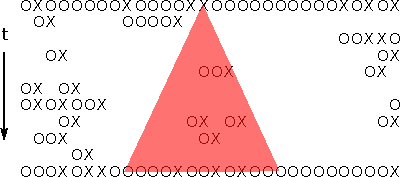
\includegraphics[width=\textwidth]{../../../writeup-plots/talk-tasep-fig-3}

    \end{column}
  \end{columns}

\end{frame}



% e^tG; previous work
\begin{frame}{Idealized solution}

  This is a continuous-time, finite-state Markov chain on length-$n$ sequences.
  
  \vspace{1em}

  Exact likelihood function, \\
  for observing sequnce $x$ evolve into $y$ in time $t$:
  \begin{align*}
    \P\{ X_t = y | X_0 = x \} = \left( e^{tG} \right)_{xy} .
  \end{align*}

  \vspace{1em}

  {\newthing Problem:} $G$ is a $4^n \times 4^n$ matrix.

\end{frame}


\begin{frame}{Previous work}

  \begin{itemize}

    \item Assume a $k$th order Markov model along the sequence \\
      -- Siepel \& Haussler 2003

    \item Expansion of $e^{tG}$ \\
      -- Lunter \& Hein 2004 

    \item Data augmentation: MCMC over true mutational path \\
      -- Hobolth 2008, Baele et al 2010

  \end{itemize}

\end{frame}

% Assumptions and not
\begin{frame}{Assumptions}

  I assume:
  \begin{itemize}

    \item homogeneity along the sequence

  \end{itemize}

  \vspace{2em}

  I do not assume:
  \begin{itemize}

    \item stationarity

    \item reversibility

  \end{itemize}

  \vspace{2em}

  Example: GC-content need not be at equilibrium.

\end{frame}


%%%%%%%%% METHODS
\section{Statistical \& Computational Methods}

%   restrict to pattern frequencies: partial likelihood
\begin{frame}{Larger windows?}

  \begin{columns}[c]
    \begin{column}{.4\textwidth}

  First attempt:
  \begin{itemize}

    \item Pick a window size $w$

    \item Count all pairs of $w$-tuples: \\
      $n(a,b) = \# \{ a \to b \}$ \\
      {\aside (nonoverlapping?)}

    \item Compute $4^w \times 4^w$ transition matrix $G_w$.

  \end{itemize}

  \vspace{2em}

  Assume each $w$-window evolves indpendently --
  partial/pseudo-likelihood: 
  \begin{align*}
    \mathcal{L} = \prod_{a,b} n(a,b) \log \left( e^{tG_w} \right)_{ab} .
  \end{align*}

    \end{column}
    \begin{column}{.6\textwidth}

      Example: $w=3$
      \only<1>{
            {
          \begin{center} \setlength{\tabcolsep}{0pt} \begin{tabular}{cccccccccccccccccccccccccccccccccccccccccccccccccccccccccc}
            \cline{1-3}
            \tLL{C}&C&\tRR{C}&A&G&T&C&C&A&G&A&T&A&A&A&A&T&T&G&A&T&A&A&C&T&C\\
            \tLL{C}&A&\tRR{C}&A&G&T&C&C&A&G&A&T&A&A&A&A&T&C&G&A&T&A&A&C&T&C\\
            \cline{1-3}
          \end{tabular} \end{center} 
          }
      }
      \only<2>{
            {
          \begin{center} \setlength{\tabcolsep}{0pt} \begin{tabular}{cccccccccccccccccccccccccccccccccccccccccccccccccccccccccc}
            \cline{4-6}
            C&C&C&\tLL{A}&G&\tRR{T}&C&C&A&G&A&T&A&A&A&A&T&T&G&A&T&A&A&C&T&C\\
            C&A&C&\tLL{A}&G&\tRR{T}&C&C&A&G&A&T&A&A&A&A&T&C&G&A&T&A&A&C&T&C\\
            \cline{4-6}
          \end{tabular} \end{center} 
          }
      }
      \only<3>{
            {
          \begin{center} \setlength{\tabcolsep}{0pt} \begin{tabular}{cccccccccccccccccccccccccccccccccccccccccccccccccccccccccc}
            \cline{7-9}
            C&C&C&A&G&T&\tLL{C}&C&\tRR{A}&G&A&T&A&A&A&A&T&T&G&A&T&A&A&C&T&C\\
            C&A&C&A&G&T&\tLL{C}&C&\tRR{A}&G&A&T&A&A&A&A&T&C&G&A&T&A&A&C&T&C\\
            \cline{7-9}
          \end{tabular} \end{center} 
          }
      }

      \vspace{2em}

      {\struct but:} still misses edge effects.



    \end{column}
  \end{columns}
\end{frame}


%   still missing edge effects: marginalize over window
%     node average boundary
\begin{frame}{Still missing those edge effects}

  \begin{columns}[c]
    \begin{column}{.4\textwidth}

      {\newthing Solution:} Trim the bottom window.

      \vspace{1em}

      Count pairs of $(w,r)$-tuples, with $r<w$,

      \vspace{1em}

      computing the probability of a change by marginalizing over the omitted bases.

      \vspace{1em}

  Must still deal with nonindependence --
  partial/pseudo-likelihood: 
  \begin{align*}
    \mathcal{L} = \prod_{a,c} n(a,c) \sum_{b \supset c} \log \left( e^{tG_w} \right)_{ab} .
  \end{align*}

    \end{column}
    \begin{column}{.6\textwidth}

      Example: $w=3,r=1$
      \only<1>{
            {
          \begin{center} \setlength{\tabcolsep}{0pt} \begin{tabular}{cccccccccccccccccccccccccccccccccccccccccccccccccccccccccc}
            \cline{1-3}
            \tLL{C}&C&\tRR{C}&A&G&T&C&C&A&G&A&T&A&A&A&A&T&T&G&A&T&A&A&C&T&C\\
            \cline{1-1}\cline{3-3}
            C&\tLR{A}&C&A&G&T&C&C&A&G&A&T&A&A&A&A&T&C&G&A&T&A&A&C&T&C\\
            \cline{2-2}
          \end{tabular} \end{center} 
          }
      }
      \only<2>{
            {
          \begin{center} \setlength{\tabcolsep}{0pt} \begin{tabular}{cccccccccccccccccccccccccccccccccccccccccccccccccccccccccc}
            \cline{4-6}
            C&C&C&\tLL{A}&G&\tRR{T}&C&C&A&G&A&T&A&A&A&A&T&T&G&A&T&A&A&C&T&C\\
            \cline{4-4}\cline{6-6}
            C&A&C&A&\tLR{G}&T&C&C&A&G&A&T&A&A&A&A&T&C&G&A&T&A&A&C&T&C\\
            \cline{5-5}
          \end{tabular} \end{center} 
          }
      }
      \only<3>{
            {
          \begin{center} \setlength{\tabcolsep}{0pt} \begin{tabular}{cccccccccccccccccccccccccccccccccccccccccccccccccccccccccc}
            \cline{7-9}
            C&C&C&A&G&T&\tLL{C}&C&\tRR{A}&G&A&T&A&A&A&A&T&T&G&A&T&A&A&C&T&C\\
            \cline{7-7}\cline{9-9}
            C&A&C&A&G&T&C&\tLR{C}&A&G&A&T&A&A&A&A&T&C&G&A&T&A&A&C&T&C\\
            \cline{8-8}
          \end{tabular} \end{center} 
          }
      }

      {\struct Ex:} 
      \begin{align*}
        & \P\{\text{CCC} \to \cdot\text{A}\cdot\} = \\
        &\quad \P\{\text{CCC} \to \text{CAC} \} \\
        &\qquad {}+\P\{\text{CCC} \to \text{CAA} \}  \\
        &\qquad {}+\P\{\text{CCC} \to \text{CAG} \}  \\
        &\qquad {}+\P\{\text{CCC} \to \text{GAC} \}  \\
        &\qquad {}+\P\{\text{CCC} \to \text{GAT} \}  \\
        & \qquad {} + \cdots 
      \end{align*}



    \end{column}
  \end{columns}

\end{frame}


%   asymptotically correct: propagation of dependency
\begin{frame}{Asymptotic correctness}
  \begin{columns}[c]
    \begin{column}{.4\textwidth}

  {\struct Claim:} \\
  If the size of the trimmed window is large enough, this is a {\newthing correct} (partial) likelihood.

    \end{column}
    \begin{column}{.6\textwidth}

  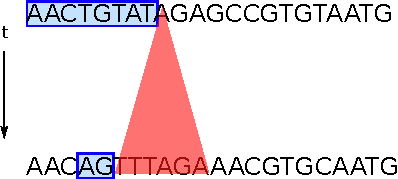
\includegraphics{../../../writeup-plots/talk-dependency-proof-fig}

    \end{column}
  \end{columns}

\end{frame}

%   likelihood function
\begin{frame}{Inference framework: likelihood function}

  single branch; time is confounded with mutation

  given parameters:
    
    mutation patterns

    selection patterns (and form)


  and:

    set of patterns

    set of positions


  likelihood is: (multinomial)

\end{frame}

%   computation: sparse matrices
\begin{frame}{Computation: using sparseness}

\end{frame}

%   phylogenetic peeling (?)
\begin{frame}{Larger phylogenies}

\end{frame}


%%%%%%%%% APPLICATIONS
\section{Applications}

%   CpG
\begin{frame}{Nucleotide sequence}

\end{frame}

%   TASEP
\begin{frame}{Propagation of dependency: TASEP}

\end{frame}

%   Ising
\begin{frame}{Statistical physics: the Ising model}

\end{frame}

%   real data?
\begin{frame}{Real data}

  still running\ldots

\end{frame}

%   ancestral state reconstruction
\begin{frame}{Other applications}

  Ancestral state reconstruction

  Ancestral methylation inference

\end{frame}

%%%%% ok all done

\begin{frame}{Thanks}

  Matt Dean
  
  Rasmus Nielsen

  Simon Tavar\'e

  Graham Coop

  Sergey Nudzhin

\end{frame}

\end{document}
